\documentclass[12pt,twoside,openright]{book}

\usepackage{styles/rbruacademic}

\begin{document}

% -------------------------------------------------------------
% หน้าปก 3D Farmer Outfit with Sleeve Logo (v13 Standalone Cover A4)
% -------------------------------------------------------------
\begin{titlepage}
\newgeometry{margin=0pt}
\thispagestyle{empty}
\begingroup
\setlength{\XeTeXlinebreakskip}{0pt}
\begin{tikzpicture}[remember picture, overlay]
    % 1. Full-Bleed 3D Cover Artwork (A4: 210 x 297 mm)
    \node[anchor=center, inner sep=0pt] at (current page.center) {
        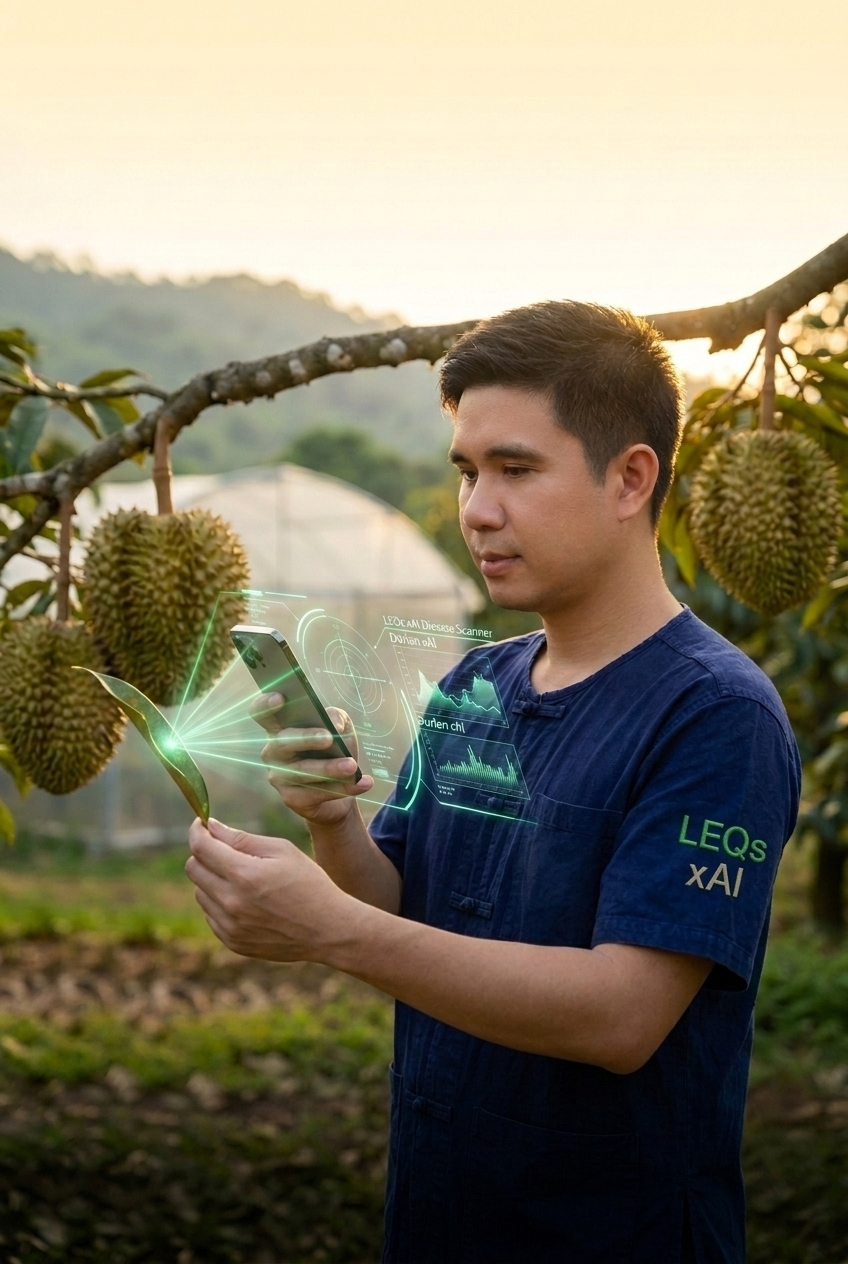
\includegraphics[width=\paperwidth,height=\paperheight]{figures/cover_v13_chewa_farmer_sleeve_leqsxai.jpg}
    };

    % 2. UPPER SKY ZONE: Transparent Architecture with Dual-Layer Micro Drop-Shadow
    % Shadow Layer (Soft white glow halo for crisp contrast against bright sky)
    \node[anchor=north, align=center, text width=7.2in] at ([xshift=0.5pt, yshift=-0.16in]current page.north) {
        \begin{tikzpicture}
            \node[fill=deepIndigo!85, text=white, rounded corners=2.5mm, inner sep=4.5pt, font=\fontsize{9.5}{12}\selectfont\bfseries] {
                \color{cyberCyan}$\blacktriangleright$\ \color{white}SMART AGRICULTURE \& EDGE AI MOBILE SERIES\ \color{neonEmerald}$\blacktriangleleft$
            };
        \end{tikzpicture}\\[4pt]
        {\fontsize{11}{14}\selectfont\color{white}\textbf{เอกสารคำสอนและคู่มือปฏิบัติการขั้นสูง \textbullet\ มหาวิทยาลัยราชภัฏรำไพพรรณี}}\\[5pt]
        
        % Main Title Line 1
        {\fontsize{26}{32}\selectfont\bfseries\color{white} การออกแบบและพัฒนาแอปพลิเคชันสมาร์ทโฟน}\\[3pt]
        % Main Title Line 2
        {\fontsize{34}{42}\selectfont\bfseries\color{white} วิเคราะห์โรคในทุเรียน}\\[5pt]
        % Beginner Pill Tag
        \begin{tikzpicture}
            \node[draw=cyberCyan, line width=1.2pt, rounded corners=2.5mm, inner sep=4.5pt] {
                \fontsize{14}{18}\selectfont\bfseries\color{white} สำหรับผู้เริ่มต้นไม่มีพื้นฐานการเขียนโค้ด
            };
        \end{tikzpicture}\\[6pt]
        % English Subtitle
        {\fontsize{10.5}{13.5}\selectfont\bfseries\color{white} DESIGN AND DEVELOPMENT OF SMARTPHONE APPLICATION FOR DURIAN DISEASE ANALYSIS}\\[2.5pt]
        {\fontsize{9.5}{12.5}\selectfont\color{white} (A NO-CODE \& BEGINNER-FRIENDLY GUIDE TO COMPUTER VISION \& EDGE AI)}
    };

    % Foreground Layer (Crisp typography floating directly on transparent background)
    \node[anchor=north, align=center, text width=7.2in] at ([yshift=-0.165in]current page.north) {
        \begin{tikzpicture}
            \node[fill=deepIndigo!90, text=white, rounded corners=2.5mm, inner sep=4.5pt, font=\fontsize{9.5}{12}\selectfont\bfseries] {
                \color{cyberCyan}$\blacktriangleright$\ \color{white}SMART AGRICULTURE \& EDGE AI MOBILE SERIES\ \color{neonEmerald}$\blacktriangleleft$
            };
        \end{tikzpicture}\\[4pt]
        {\fontsize{11}{14}\selectfont\color{deepIndigo!90}\textbf{เอกสารคำสอนและคู่มือปฏิบัติการขั้นสูง \textbullet\ มหาวิทยาลัยราชภัฏรำไพพรรณี}}\\[5pt]
        
        % Main Title Line 1
        {\fontsize{26}{32}\selectfont\bfseries\color{deepIndigo} การออกแบบและพัฒนาแอปพลิเคชันสมาร์ทโฟน}\\[3pt]
        % Main Title Line 2
        {\fontsize{34}{42}\selectfont\bfseries\color{agriGreen!90!black} วิเคราะห์โรคในทุเรียน}\\[5pt]
        % Beginner Pill Tag
        \begin{tikzpicture}
            \node[draw=cyberCyan!90, line width=1.2pt, fill=white!40, fill opacity=0.3, text opacity=1.0, rounded corners=2.5mm, inner sep=4.5pt] {
                \fontsize{14}{18}\selectfont\bfseries\color{deepIndigo} สำหรับผู้เริ่มต้นไม่มีพื้นฐานการเขียนโค้ด
            };
        \end{tikzpicture}\\[6pt]
        % English Subtitle
        {\fontsize{10.5}{13.5}\selectfont\bfseries\color{deepIndigo!90} DESIGN AND DEVELOPMENT OF SMARTPHONE APPLICATION FOR DURIAN DISEASE ANALYSIS}\\[2.5pt]
        {\fontsize{9.5}{12.5}\selectfont\color{deepIndigo!75} (A NO-CODE \& BEGINNER-FRIENDLY GUIDE TO COMPUTER VISION \& EDGE AI)}
    };

    % 3. BOTTOM ZONE: 100% Transparent Architecture with Dual-Layer Micro Drop-Shadow
    % Shadow Layer
    \node[anchor=south, align=center, text width=7.0in] at ([xshift=0.5pt, yshift=0.30in]current page.south) {
        {\fontsize{18}{23}\selectfont\bfseries\color{black!90} ผู้ช่วยศาสตราจารย์ ดร.ชีวะ ทัศนา}\\[4pt]
        {\fontsize{12}{15.5}\selectfont\bfseries\color{black!90} สาขาวิชาปัญญาประดิษฐ์เพื่อเกษตรดิจิทัลและสิ่งแวดล้อม คณะวิทยาศาสตร์และเทคโนโลยี}\\[3pt]
        {\fontsize{11.5}{15}\selectfont\bfseries\color{black!90} มหาวิทยาลัยราชภัฏรำไพพรรณี \textbullet\ พ.ศ. 2569}
    };
    % Foreground Layer
    \node[anchor=south, align=center, text width=7.0in] at ([yshift=0.305in]current page.south) {
        {\fontsize{18}{23}\selectfont\bfseries\color{white} ผู้ช่วยศาสตราจารย์ ดร.ชีวะ ทัศนา}\\[4pt]
        {\fontsize{12}{15.5}\selectfont\bfseries\color{white!95} สาขาวิชาปัญญาประดิษฐ์เพื่อเกษตรดิจิทัลและสิ่งแวดล้อม คณะวิทยาศาสตร์และเทคโนโลยี}\\[3pt]
        {\fontsize{11.5}{15}\selectfont\bfseries\color{techAmber} มหาวิทยาลัยราชภัฏรำไพพรรณี \textbullet\ พ.ศ. 2569}
    };
\end{tikzpicture}
\endgroup
\end{titlepage}
\restoregeometry

\end{document}
